\documentclass[11pt, a4paper]{article}
\usepackage[latin1]{inputenc}
\usepackage{pgfplots}
\usepackage{pgfplotstable}
\usepackage{float}
\pgfplotsset{width=0.85\textwidth ,compat=1.9}
\usepackage[dutch]{babel}
\usepackage{csquotes}
\usepackage{amsmath}
\usepackage[toc,page]{appendix}
\usepackage{amsfonts}
\usepackage{amssymb}
\usepackage{graphicx}
\usepackage{caption}
\usepackage[backend=biber, style=numeric, citestyle=numeric-comp, sorting = none]{biblatex}
\author{Stef Tweepenninckx, r0677232}
\title{Practicum 1: Sorteeralgoritmes}


%define printtitle
\makeatletter
\def\printtitle{                 
    {\large \@title}} 
\makeatother

%define printauthor
\makeatletter                       
\def\printauthor{                  
    {\large \@author}}              
\makeatother

\begin{document}
\begin{titlepage}
\newcommand{\HRule}{\rule{\linewidth}{0.5mm}} 
\center 
\textsc{\LARGE Gegevensstructuren en algoritmen}\\[1.5cm] 
\HRule \\[0.4cm]

{\huge \bfseries \printtitle}\\[0.4cm] 
\HRule \\[0.4cm]

\Large \emph{Author:}\\
 \textsc{\printauthor}\\[3cm]

{\large \textsc{1 mei 2018}}\\[3cm] 

\vfill 
\end{titlepage}

\section*{Inleiding}
%TODO


\newpage
\section*{Overzicht}
\begin{table}[ht]
\centering
\label{my-label}
\begin{tabular}{|cccc|}
\hline
Puzzel       & Aantal vergelijkingen & Hamming (s)        & Manhattan (s) \\ \hline
puzzle28.txt & 28                    & 2.435              & 0.113         \\
puzzle30.txt & 30                    & 3.920              & 0.140         \\
puzzle32.txt & 32                    & \textgreater 5 min & 4.803         \\
puzzle34.txt & 34                    & \textgreater 5 min & 1.093         \\
puzzle36.txt & 36                    & \textgreater 5 min & 14.168        \\
puzzle38.txt & 38                    & \textgreater 5 min & 10.885        \\
puzzle40.txt & 40                    & \textgreater 5 min & 2.490         \\
puzzle42.txt & 42                    & \textgreater 5 min & 8.528         \\ \hline
\end{tabular}
\captionsetup{justification=centering,margin=2cm}
\caption{Resultaten experiment met Hamming en Manhattan prioriteitsfunctie}
\end{table}
\section*{Tijdscomplexiteit Hamming}
De Hamming prioriteitsfunctie kijkt naar het aantal elementen die op de foute plaats staat. We lopen over de hele puzzel en vergelijken de waarde op een bepaalde positie i,j met de verwachte waarde. Als deze 2 waarden niet overeenkomen verhogen we het resultaat.\\
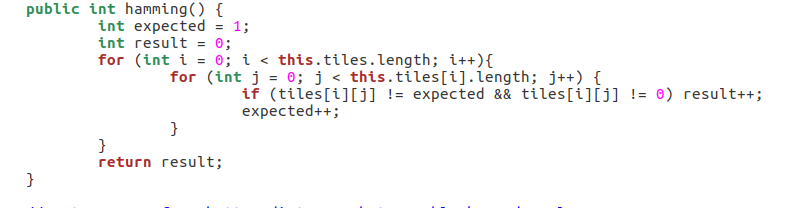
\includegraphics[width=\textwidth]{hamming}\\
In mijn implementatie van de Hamming functie gebruik ik twee for-lussen die beide van 0 tot N lopen. Bij elke iteratie zijn er maximaal twee array accesses nodig. In dit worst-case geval is de tijdscomplexiteit $\sim 2N^2$.\\
In het beste geval (de puzzel is al opgelost) wordt de 2\textsuperscript{e} array access slechts 1 keer uitgevoerd, bij het 0-vakje (dit kan nooit gelijk zijn aan de variabele \emph{expected}). Bij de gewone vakjes is de if-clausule al gefalsifi\"eerd door de 1\textsuperscript{e} array access en wordt de 2\textsuperscript{e} dus niet uitgevoerd. De best-case tijdscomplexiteit is dus $\sim N^2 + 1$.
%TODO average case

\section*{Tijdscomplexiteit Manhattan}
De Manhattan prioriteitsfunctie kijkt naar de totale afstand tussen de elementen en hun juiste locatie. We lopen over de hele puzzel en vergelijken de waarde op een bepaalde positie i,j met de verwachte waarde. Als deze 2 waarden niet overeenkomen berekenen we de afstand tot de juiste positie en verhogen we het resultaat met deze afstand.\vspace*{10px}
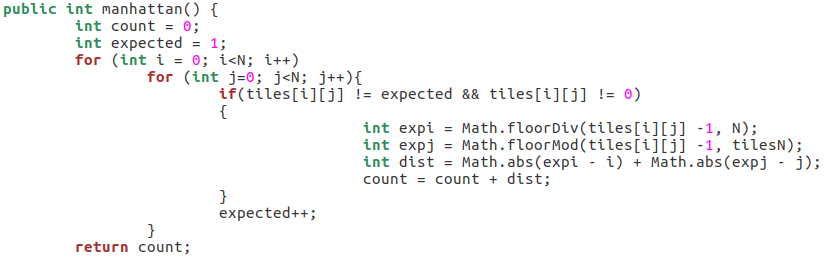
\includegraphics[width=\textwidth]{manhattan}\\
\captionof{figure}{Implementatie van Manhattan prioriteitsfunctie}
\vspace*{10px}
Net als bij de Hamming functie, gebruikt mijn Manhattan functie twee for-lussen die van 0 tot N lopen. Bij elke iteratie zijn er maximaal 4 array accesses nodig. De worst-case tijdscomplexiteit is dus $\sim 4N^2$.\\
In het beste geval worden de binnenste array accesses nooit uitgevoerd en worden enkel bij het 0-vakje beide accesses van de if-clausule uitgevoerd. In het best-case geval is de tijdscomplexiteit dus $\sim N^2 + 1$.

\newpage
\section*{isSolvable}
In het eerste deel van isSolvable() localiseer ik het lege 0-vakje en verplaats het naar de juiste i locatie en de juiste j locatie: $i=N-1$, $j=N-1$.\\
In het tweede deel bereken ik de formule zelf met behulp van twee for-loops. Bij elke iteratie bereken ik de teller en noemer en vermenigvuldig het deeltal met het voorgaande resultaat. Op deze manier kan je de productfunctie berekenen. Op het einde return je of het resultaat groter of gelijk is dan 0 en het bord dus al dan niet oplosbaar is.\\
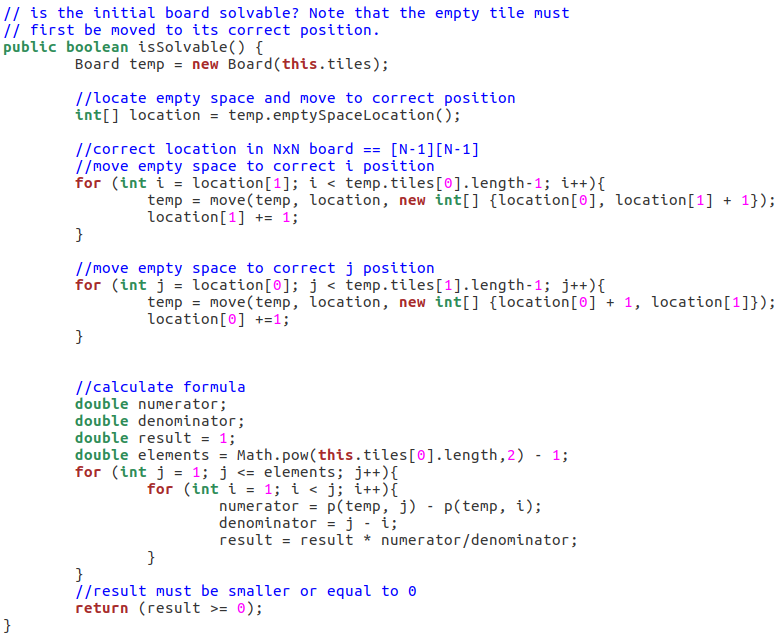
\includegraphics[width=\textwidth]{isSolvable}\\
%TODO tijdscomplexiteit isSolvable

In mijn implementatie gebruik ik 1 hulpfunctie \emph{move} om de blokjes te verschuiven. In het gemiddelde geval (0-vakje staat in het midden) wordt deze methode N keer uitgevoerd met 2 array accesses, dus een gemiddelde tijdscomplexiteit van $\sim 2N$.

\section*{Borden in geheugen}
Elk bord met grootte $N \times N$ heeft maximaal $N^2$! permutaties/verschillende bordconfiguraties. Niet alle permutaties zijn bereikbaar vanuit de initi\"ele configuratie, slechts de helft kan bereikt worden met legale verschuivingen. Het maximaal aantal bordconfiguraties in het geheugen is dus gelijk aan $\frac{N^2!}{2}$. De keuze van prioriteitsfunctie zou dit eventueel nog kunnen verlagen.
	
\section*{Worst-case tijdscomplexiteit}
De built-in priorityqueue van Java die ik gebruikt heb, heeft een complexiteit van $O(log(N))$ om een element aan de rij toe te voegen. In de vorige vraag hebben we vastgesteld dat er maximaal $\frac{N^2!}{2}$ bordconfiguraties in het geheugen zitten. Dit impliceert dat het volgende toe te voegen bord moet worden vergeleken met $log(\frac{N^2!}{2})$ borden. De gekozen prioriteitsfunctie (Hamming of Manhattan) bepaalt mee de complexiteit van de vergelijking. De worst-case complexiteit is dan:
\\
	\begin{align}
	\centering
		&log(\frac{N^2!}{2}) * 1.5N^2 * 2 \\
	=   & 3log(\frac{N^2!}{2})*N^{2} \\
	=	& 3N^2*(log(N^2!)-log(2)) \\
	=   & 3N^2*(log(N^2!)-1) \\
	=   & 3N^2*log(N^2!) - 3N^2
	\end{align}
	Met behulp van Stirling's benadering $log_2(n!) \approx nlog_2(n) - log_2(e)n + O(log_2(n))$ bekomen we:
	\begin{align}
	\centering
		& 3N^2*log(N^2!) \\
	=\sim	& 3N^2*N^2log(N^2)\\
	=\sim	& 6N^4log(N)
	\end{align}
	\\
Het verwijderen van een element met de laagste priority uit de priorityqueue gebeurt in constante tijd, het staat immers vooraan in de queue. Elk ander element gebeurt in lineaire tijd. 
\section*{Betere prioriteitsfuncties}

	
\newpage
\section*{Tijd, geheugen of algoritme?}
Een betere prioriteitsfunctie heeft naar mijn mening het meeste invloed. Dit kunnen we bijvoorbeeld zien bij de experimenten in vraag 1: met de Hamming functie zijn 6 van de 8 borden niet oplosbaar binnen de 5 minuten, terwijl de Manhattan functie een maximale tijd van 14.2 seconden heeft. Dit toont de invloed van een goed algoritme op de effici\"entie.\\
Dat meer tijd niet de beste manier is kunnen we op dezelfde manier aantonen: de langste tijd met Manhattan is 14.2 seconden, hetzelfde bord met Hamming is meer dan 5 minuten. 10 keer zo veel tijd heeft dus amper invloed op een probleem met deze complexiteit.\\
Meer geheugen is ook niet de oplossing, aangezien een betere prioriteitsfunctie impliceert dat er minder borden in de priorityqueue zitten en dus ook minder geheugen nodig heeft.
	
\section*{Effici\"ent algoritme}
%TODO
	


\end{document}
